\chapter{Implementation}


\section{Implementation Language Choice}

The compiler will be implemented using the Haskell programming language.

During complication the need to traverse trees usually occurs quite
often. Functional languages like Haskellare suited to this task 
due to features such as pattern matching and tail-end recursive optimisation 
which make traversing trees efficient and simple to implement/ 

The Glasgow Haskell Compiler is available for most platforms, most importantly for Windows, OSX and Linux 
on x86 architectures. This allows the compiler to be portable across these platforms provided the libraries 
used to build the compiler are portable.

Haskell has algebaric datatypes, these makes Abstract Syntax Trees
simpler to implement. For example the AST for a very simple expression
can be representedas follows:

\begin{lstlisting}[style=myHaskell]

    data Expression =
          Add Expression Expression
        | Negate Expression 
        | Const Integer

\end{lstlisting}

The equivalent in an Imperative/OOP language (in this case Java)
would be the following:

\begin{lstlisting}[style=myJava]

abstract Class Expression {}

class Add extends Expression {
    public Expression left;
    public Expression right;
    public Add(Expression l, Expression r) {
        left = l;
        right = r;    
    } 
}

class Negate extends Expression {
    public Expression expr;
    public Negate(Expression e) {
        expr = e;    
    }
} 

class Const extends Expression {
    public int value;
    public Const(int v) {
        value = v;
    }
}       

\end{lstlisting}

The Haskell version is much clearer on the structure of the tree, and takes much
less code to implement. 

It is also to easily extend Haskell datatypes to include
custom annotations. For example storing the source code position for parts of expressions may
be useful for reporting errors to the user.

Due to the pure function nature of Haskell, parts of complilation can easily be performed in parallel.
For example during type checking, each GPC function can be type checked in parallel and this can even be subdivided 
further into blocks within functions. For this project speed of compilation is not a major concern, but in the future if compliation ever
needs to be faster then this option is always available.

Haskell also has powerful libraries for parsing source code such as Parsec which is a parser combinator
library. Parsec allows Combinator parsers to be written in the Haskell language itself avoiding the complexity
of integration of different tools and languages\cite{parsec}. 

\section{Tools and Testing}


\subsection{Cabal}

Cabal (Common Architecture for Building Applications and Libraries) is a system for building and
packaging Haskell libraries and programs.\cite{cabal}. This system can manage the
project library dependencies, and automatically download and install missing dependencies.
It can also build amd install the compiler on the system, and run unit tests.

\subsection{Testing}

For Unit testing the HUnit library will be used, this can be integrated
with Cabal to easily run all the required unit tests.

One form of testing used for this project is testing each individual component
(e.g. The Parser or the TypeChecker). Each component in the compiler can easily
be uncoupled from one another due to the linear nature of compliation.

Another form of testing is writing GPC source files which should compile, and
GPC files which should fail compilation at a certain stage. The compiler
is then invoked during testing on all of these files to check whether
all the source files which should compile do infact compile with no errors,
and all the source files which should raise an error do not compile.

An upside to this method is that testing this way is flexible in that
they aren't coupled with the implementation internals of the compiler.
The only way that these test would need to be changed was if the design
of the language itself would need to be changed.

The downsides to this method is that without manually checking the errors raised
by the tests that should fail the source may generate an error which is unrelated
to the error that is being tested. This is why some testing of each internal
component is done alongside this method.

\subsection{Code Coverage}

The Haskell HPC (Haskell Program Coverage) library allows for recording
code coverage over different modules during testing. This can be integrated with
cabal unit testing to automatically generate these results. The usefulness of this
allows for checking which sections of code still need to be tested and assists
in writing further unit tests.


\section{Compiler Structure}
Compilation is split up into multiple stages or "passes",
it is possible to compile in one pass but seperating each 
specific section of compilation allows modularity and decoupling.

\newpage
\begin{figure}[!htb]
\begin{center}
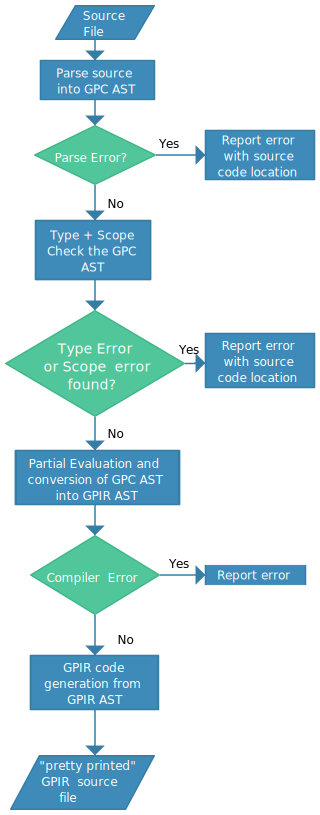
\includegraphics{graphs/Dissertation.pdf}
\caption{Flowchart illustrating the stages of the GPC compiler.}
\end{center}
\end{figure}

    
\subsection{Parser/Lexer}
The Parsec library combines Parsing and Lexing into one stage.

Given the GPC source file the intention is to parse the file into an AST
to hopefully eventually be transformed into GPIR source code. It's
also useful to store the original source position to provide error information 
during a further compilation stage, to achieve this the source position
info is read from Parsec into an Annotated AST as the tree is being built up.

Parsec does most of the work during this stage, including
providing error messages for "expected" values to be found in source
positions and source position information. Most of the work implementing
this stage is building the parser combinator functions and composing
them together to be able to build the AST.


\subsection{Type and Scope checking}

During type checking the types of identifiers from the current scope being used in expressions need
to be known. Since the scope needs to be kept track of while type checking it makes reasonable
sense to check for scope errors in the same stage.

The goal of this stage is to ensure that the static typing of the source file
is enforced (e.g. attempting to assign a bool value to a variable of type int should not happen) and,
prevent "logic" errors at compile time (e.g. adding 2 bool values together). Scope checking
is also important as identifiers being used within the program need to be binded to an expression of
some sort, and the "single assignment" rule in the GPC language needs to be enforced.

There are two seperate "types" of scope in a GPC program. The first is the top level scope and the
other is at function level scope. Any scope "further" down from function level scope is itself
a function level scope. During this stage the top level scope will be type and scope checked.
Afterwards each individual function will be type and scope checked.

For checking over top level statements the following Haskell record is used
to keep track of identifier types, objects, and functions encountered:

\begin{lstlisting}[style=myHaskell]
type VarTable = M.Map (Ident SrcPos) (Type SrcPos)
type FunTable = M.Map (Ident SrcPos) (Type SrcPos, [Type SrcPos])
type ObjectTable = M.Map (Ident SrcPos) (Objects SrcPos)

data MainBlock = MainBlock {
    _tlFuncDefs      :: FunTable, -- ^ Function Definitions
    _tlVarTypes      :: VarTable,  -- ^ Top Level Constant variable types
    _objects         :: ObjectTable  -- ^ Table of current Kernel objects declared 
} deriving (Show)
\end{lstlisting}

It needs to be checked that no duplicate functions exist and  no duplicate top level variables exist,
Once all top level statements have been checked, all functions in scope stored, 
all top level variables stored, and all variables stored. Each individual function
can be checked.

A slightly different stucture is needed to type check functions.

At anytime it is needed to be known what variables that are currently in scope, their types,
what functions are avilable to call, their argument types, and return types. Also the
objects which are available to call methods on, and the current function the type checker
is in at any point.

These values can be stored using the following Haskell record: 

\begin{lstlisting}[style=myHaskell]

data CodeBlock = CodeBlock {
    _currentFun :: Ident SrcPos, -- ^ Name of Function block is in
    _funcDefs   :: FunTable, -- ^ Function names and return/argument types
    _prevVars   :: VarTable, -- ^ Identifiers visible in current scope with types
    _curVars    :: VarTable  -- ^ Identifiers declared in current scope
} deriving (Show)


\end{lstlisting}

When a function is being type check a new CodeBlock instance needs to be
created from a MainBlock instance, as some of the top level information is needed.
The details of the function that is being entered is stored in "\_currentFun", 
details of all available functions stored in "\_funcDefs", and store all
top level variable in "\_prevVars". "\_curVars" is left as an empty map as the
type checking of the function hasn't begun yet. Top level objects are also
stored in "\_curVars" as an "object" variable type.

Whenever a new scope is encountered by either calling a function, or entering a seq/par block;
A new CodeBlock structure is created using the current structure. The new "\_curVars"
is set to the empty map as no variables have been encountered yet, the "\_funcDefs"
are copied as all functions are on the top level so they don't change. The "\_currentFun"
is copied if entering a block, otherwise if entering a function the function name
and source position are copied. 

The value of the new "\_prevVars" is a little more complicated to work out.
Any key, value pairs in the current "\_curVars" are stored plus any key, value
pairs in the current "\_prevVars" in which the key isn't present in the current 
set of "\_curVars" keys. This is because
the identifiers in "\_curVars" scope are visible over the identifiers with
the same name in "\_prevScope". Haskell's union operation on maps
discards the key, value pairs in the second map for keys that are
present in the first map, so this is trivial to implement.

When type checking a function, every statement in the function is type checked
as well as the type of the return statement. For every statement,
every expression within the statement is type checked. This is implemented by traversing
the Statement AST and checking the scopes of identifiers as well as expected types
against actual types.

Objects which are declared are not checked to see if they actually exist. Neither
are method calls which means the argument types and return types when calling them
cannot be determined at compile time. This is due to the fact Objects are written
in C++, and the C++ class would need to be checked for methods and types. This is already
implemented in the GPRM, so an error will occur further down to compile "chain" or during
runtime.

If a type or scope error is encountered, an error message determining the type of error,
and the source position of the error is returned. Otherwise an empty tuple is returned.
When type and scope checking the original AST doesn't need to be modified, only verified
that it follows the type and scope rules of the language.


\subsection{Evaluation}

The goal of this stage is to run through the execution path the GPIR code
will take from the entry function, and partially evaluate the code as much
as possible while generating the GPIR AST.

Just before Evaluation the AST is transformed slightly into a similar AST
with two differences. One is that annotations are not present (since source position information
is not needed anymore), and type information is stripped (since the program has been proven to 
not have any type errors).




\begin{lstlisting}[style=myHaskell]

type ConstVarTable = M.Map Ident Literal
type FunTable = M.Map Ident ([Ident], BlockStmt)
type VarRegTable = M.Map Ident Integer

-- ^ Current State of the Block we are currently in
data CodeGen = CodeGen {
   _funTable    :: FunTable,  -- ^ Store symbol tree for functions
   _constTable  :: ConstVarTable, -- ^ Store constants in scope
   _varId       :: Integer, -- ^ Current variable id for mapping to registers
   _varRegTable :: VarRegTable, -- ^ maps variable identifier
   _threadCount :: Integer, -- ^ Current thread number to map
   _maxThreads  :: Integer,  -- ^ Maximum number of threads
   _seqBlock    :: Bool, -- ^ Whether or not current block is sequential
   _isReturning :: Bool -- ^ Whether the state of the current block is in a return
}

\end{lstlisting}

\subsection{GPIR Code Generation}





